\section{Performance evaluation}%
\label{Performance}

In the following, we present the evaluation results of \name. 
We first give precisions on the evaluation testbed and parameters in section~\ref{sub:evaluation_testbed}, before evaluating the PORs creation  in section~\ref{sub:predictive_onion_routes_creation}, to conclude with an overall evaluation of the file transfer performance in section~\ref{sub:file_transfer}.

\subsection{Evaluation testbed} % (fold)
\label{sub:evaluation_testbed}

\subsubsection{Simulating user behavior} % (fold)
\label{ssub:simulating_user_behavior}


To evaluate \name, we take interest in users owning a variable amount of devices of different types, and frequently switching among them.
To the best of our knowledge, there exists no real-world dataset of the devices connection times of such a user.
We have thus implemented an evaluation testbed where each user's behavior is simulated  according to the following properties:
\begin{itemize}
	\item The user owns a variable amount of devices. We consider the following device types: mobile (e.g. tablet, phone), portable (laptop), fixed (workstation, home computer) and server (such as a NAS, Raspberry Pi or rented appliance);
	\item She can travel between different locations, say her home, her workplace and and outside;
	\item She makes a different use of her devices depending on her location: her home computer will only be accessed at home, while her phone can be accessed everywhere (though she tends to use it the most at home, for instance).
\end{itemize}

We thus model each user with a Hidden Markov Model, as presented in section~\ref{sub:a_model_of_the_user_s_behavior}.
We keep the different possible locations $\mathcal{L}$ to $N=3$ and the state transition matrix $A$ to a fixed value (cf figure~\ref{fig:hmm}).
The number and types of devices per user, along with the matrix of emission probabilities $B$, is determined randomly according to the following rules.

A user always has a phone, plus a random number of 2 to 9 devices whose type is decided by a weighted random choice: each device has 30\% chances of being either mobile, portable, or fixed, and only 10\% probability of being a server.
$B_{*, d}$, the probability that device $d$ is used in each location, depends on $d$'s device type: 
\begin{itemize}
	\item for each location, every mobile device $d_m$ has a random but high probability of being online: $\forall l \in \mathcal{L}, B_{l, d_m} \in [0.6, 1]$;
	\item a portable device $d_p$ has a much lower probability of being used: $\forall l \in \mathcal{L}, B_{l, d_p} \in [0.2, 0.8]$; 
	\item a fixed appliance $d_f$ has a non-zero probability of usage in only one location: $\exists l \in \mathcal{L}, B_{l, d_f} \in [0.4, 0.8] \text{ and } \forall l' \neq l, B_{l', d_f} = 0$;
	\item a server $d_s$ has a very high probability of working, whatever the user's location: $\exists p \in [0.9, 1], \forall l \in \mathcal{L}, B{l, d_s} = p$.
\end{itemize} 

\begin{figure}[t]
\centering
\vspace{-1em}
\footnotesize
\centering
$$A =
\kbordermatrix{
      & W   & O   & H   \cr
    W & 0.6 & 0.4 & 0   \cr
    O & 0.2 & 0.6 & 0.2 \cr
    H & 0   & 0.4 & 0.6 \\[0.3em]
}, \;
B = 
\kbordermatrix{
      & W     & O   & H   \cr
    p & 0.7 & 0.6 & 0.8 \cr
    w & 0.7 & 0   & 0   \cr
    h & 0   & 0   & 0.7 \cr
    l & 0.2 & 0.4 & 0.6 \\[0.3em]
}$$

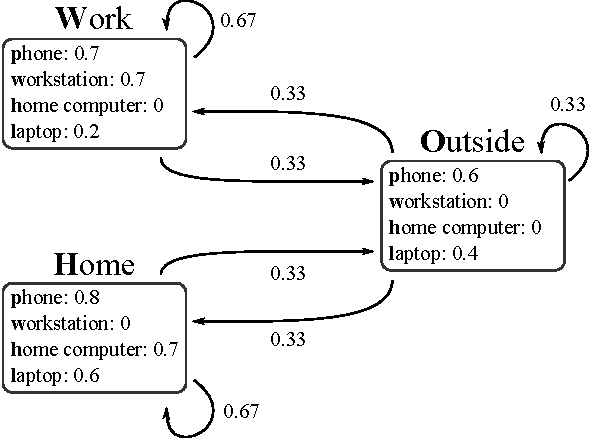
\includegraphics[width=0.65\columnwidth]{figures/hmm.pdf}
\vspace{2ex}
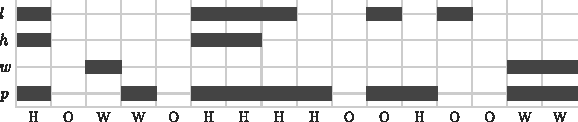
\includegraphics[width=0.9\columnwidth]{figures/sample_usage.pdf}

\caption{\label{fig:hmm} Example Hidden Markov Model (HMM) of a user's behavior: on top are the HMM parameters, on the middle is a visual representation of the model, and on the bottom is a sample output from the model.}
\end{figure}

HMMs being generative probabilistic models, they allow the generation of observation sequence $O$ given the parameters of the model $\lambda_N$.
Figure~\ref{fig:hmm} shows a possible outcome of the creation of a user's HMM $\lambda_N$, its graphical representation, along with a sample observation sequence $O$ output from the model $\lambda_N$.

Each round lasts $T=10s$ and users start at different times. 
This way, even though the round period is fixed, devices enter and leave the system at different points in the continuous time.


\subsubsection{Experimental parameters} % (fold)
\label{ssub:experimental_parameters}

In the following, we perform two types of experiments: 
section~\ref{sub:predictive_onion_routes_creation} evaluates the establishment of PORs, while section~\ref{sub:file_transfer} handles file transfer.
For that reason, they used different parameter sets.


\paragraph*{PORs creation}
Figure \ref{fig:success_rate_vs_t} come from the same data, with 10 experiments per set of settings.
$\theta$, the threshold of the probability that all nodes fail at once (cf. \ref{ssub:building_routes}), takes the following values: $[0.1, 0.01, 0.001, 0.0001]$.
$L$, the number of layers constituting a route, takes the following values: $[3, 5, 7]$.
The time since route establishment goes from 1 to 10 with  unit step.
It is measured in time periods $T$, the interval at which users change the connection state of their devices.
An experiment consisted in $L*5$ users, where we randomly picked pairs of users to compute 20 routes.
Hence, each point on the top of figure~\ref{fig:nodes_per_layer_vs_theta} is the average of 3000 layers size; 
each point on the bottom is the availability rate over 200 routes.


\paragraph*{File exchange}
In section~\ref{sub:file_transfer}, we fix the routes' creation parameters: $\theta=10^-3$, $L=3$.
The number of users is set to 20, and the number of file exchange per experiment to 10.
We use a constant file chunk size of 512kB, a constant header size of 100kB, and a constant bandwidth per link of 128kB/s.

\subsection{Predictive Onion Routes creation} % (fold)
\label{sub:predictive_onion_routes_creation}

We first measure the influence of the parameter $\theta$ on the number of nodes per layer on the top of figure~\ref{fig:success_rate_vs_t}, by displaying average and standard deviation of the number of nodes for $\theta=[10^{-4}, 10^{-3}, 10^{-2}, 10^{-1}]$ (the other experiment parameters are listed in section~\ref{ssub:experimental_parameters}).
As we can see, the number of devices per layer logarithmically decreases as we relax the constraint on the layer's availability.
The mean number of devices per layer lies between 2 and 6.
Still, the number of nodes per layer is very variable: at $\theta=10^{-4}$, values range from 2 to 11, with a standard deviation of 1.44. 

\begin{figure}[t]
\centering
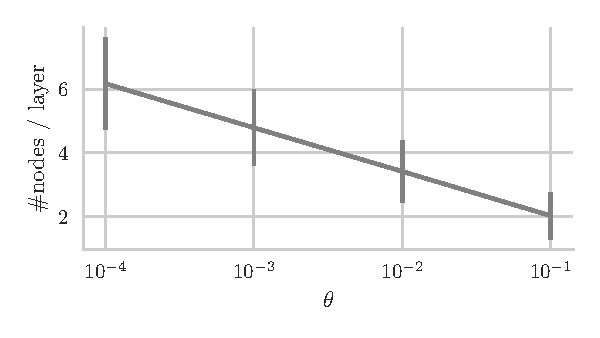
\includegraphics[width=0.7\columnwidth]{figures/nodes_per_layer_vs_theta.pdf}
\vspace{2ex}
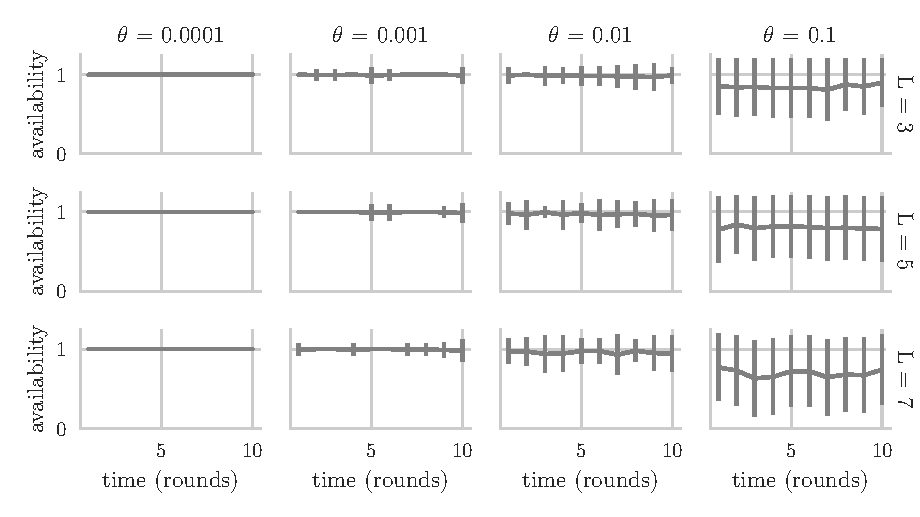
\includegraphics[width=0.9\columnwidth]{figures/success_rate_vs_t.pdf}
\caption{\label{fig:success_rate_vs_t}On top: Number of nodes per layer of POR as a function of the parameter $\theta$ (the maximal probability that all nodes in a layer fail at once). The number of nodes logarithmically decreases as we relax the $\theta$ constraint. On bottom: Availability rate of routes as a function of the time since the route establishment, for several values of the parameters $\theta$ (the maximal probability that all nodes in a layer fail at once) and $L$ (the number of layers in the route).}
\end{figure}

We now study the influence of the parameters on the future availability of the routes in figure~\ref{fig:success_rate_vs_t}.
We consider a route available if at least one node per layer is online at this time.
The plots reads the mean availability of routes as a function of the time since the route's establishment, for every couple of parameters $(\theta, L)$.
First of all, we observe that time has a negligible impact on the availability of routes. 
This shows, as was stated in section~\ref{para:predicting future behavior}, that the prediction that devices make of behavior at $t+1$ is a good enough estimator for $t+i$.
We also see that $\theta$ has a big impact on the mean availability and its variability.
Still, $\theta\in\{10^-4, 10^-3\}$ allows highly available routes with an average availability of 100\% and 99.5\% respectively.
Combined with the results from figure~\ref{fig:nodes_per_layer_vs_theta}, it means that routes will need an average of 5-6 devices per layer to be highly available.
Finally, increasing $L$ logically hinders the results when using low-availability layers.
\\

We showed that creating reliable onion routes using a backbone of unreliable nodes is feasible by using predictive algorithms.
The counterpart is that messages header size grows with the number of layers and the number of devices per layer.

Considering that most onion routing solutions use a statically defined message size to avoid information leakage, a bigger header means less space for the payload in each message. The more reliable the route, the bigger the number of messages per file. There is a trade-off between route reliability and network traffic.

\subsection{File transfer time} % (fold)
\label{sub:file_transfer}


To assess the efficiency of \name, we did several file exchanges with fixed parameters and a random file size between 5MB and 500MB.
By performing 20 experiments using the parameters described in \ref{ssub:experimental_parameters}, we obtained traces for 200 file exchanges.
All files reached their destination successfully.

\begin{figure}[t]
\centering
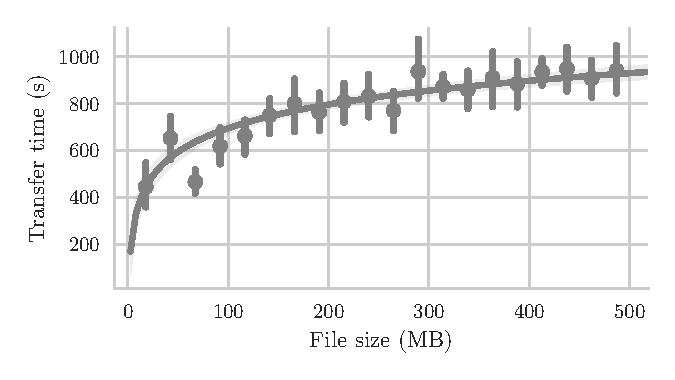
\includegraphics[width=0.7\columnwidth]{figures/transfer_time_vs_size.pdf}

\caption{\label{fig:transfer_time_vs_size}Files' transfer time as a function of their size, along with a log-linear regression of the same data.}
\end{figure}

Figure~\ref{fig:transfer_time_vs_size} shows the results of this experiment: it plots the transfer time as a function of the file size. File size is binned into 20 bins, making the series of points representing the average transfer time per bin with standard deviation bars.
We fitted a log-linear regression to this plot, displayed as a curve.
It shows that transfer time increases less fast that the file size.

Absolute time values are meaningless here: our system was evaluated on a single machine and on a single process. The code execution was not parallel, and only one device was executing at any point in time.

Still, we investigated the message transmission. In this simulation, 145172 chunks were sent, and 141276 ACKs were received: 6.00\% of the chunks were lost in transit. A chunk took an average of 56s $\pm$ 36s to reach its destination, while ACKs to 48s $\pm$ 33s to do so. This is explained mostly by devices falling offline between the time they receive a message and the time they forward it.

We now understand the log-linear curve and it's big initial slope: messages spend a long time in transit, but sending messages in parallel does not impact this time. Even small files thus need a lot of time to transfer, while bigger files do not suffer more than small files from the messages delay.
\\

Overall, we succeeded in creating a reliable and secure file transfer protocol over an underlying network of unreliable, low-end devices.
Its performance could be enhanced by taking interest in bottlenecks in the messages transmission, i.e. scheduling messages in a similar predictive manner as we planned routes creation.




% subsection file_transfer (end)